%%%%%%%%%%%%%%%%%%%%%%%%%%%%%%%%%%%%%%%%%
% University Assignment Title Page 
% LaTeX Template
% Version 1.0 (27/12/12)
%
% This template has been downloaded from:
% http://www.LaTeXTemplates.com
%
% Original author:
% WikiBooks (http://en.wikibooks.org/wiki/LaTeX/Title_Creation)
%
% License:
% CC BY-NC-SA 3.0 (http://creativecommons.org/licenses/by-nc-sa/3.0/)
% 
% Instructions for using this template:
% This title page is capable of being compiled as is. This is not useful for 
% including it in another document. To do this, you have two options: 
%
% 1) Copy/paste everything between \begin{document} and \end{document} 
% starting at \begin{titlepage} and paste this into another LaTeX file where you 
% want your title page.
% OR
% 2) Remove everything outside the \begin{titlepage} and \end{titlepage} and 
% move this file to the same directory as the LaTeX file you wish to add it to. 
% Then add \documentclass[12pt]{article}
\usepackage[english]{babel}
\usepackage{amsmath}
\usepackage{graphicx}
\usepackage{textcomp}
\usepackage{parskip}
\usepackage[colorinlistoftodos]{todonotes}
\usepackage{csquotes}
\usepackage{float}
\usepackage[backend=biber,style=ieee]{biblatex}
\addbibresource{bibliography.bib}

\begin{document}

\begin{titlepage}

\newcommand{\HRule}{\rule{\linewidth}{0.5mm}}
\center 

\textsc{\LARGE Iowa State University }\\[1.5cm] 
\textsc{\Large Center for Statistics and Applications in Forensic
Evidence
}\\[0.5cm] 

\HRule \\[0.4cm]
{ \huge \bfseries Shoe Print Data Collection: Additional Methods }\\[0.4cm] 
\HRule \\[1.5cm]



\begin{center}
\centering
 
\includegraphics[scale=.4]{csafe-logo}\\[1cm]
\end{center}







\end{titlepage}

\section{Introduction}

 When developing the methodology for the longitudinal shoe study conducted by the Center for Statistics and Applications in Forensic Evidence (CSAFE), collection procedures were designed to obtain the most ideal shoe-sole impression possible. While these images will be useful to the researcher and practitioner communities, they do not provide realistic examples of prints that would be collected from a crime scene/suspected crime scene. For this reason, CSAFE researchers have compiled this manual which contains procedures for further data collection and offers new, or edited, procedures that better represent the practices of current forensic examiners and crime scene teams. If at any time there is a question on any of these procedures, please make a note using a post-it note and e-mail the principal investigator, the project manager, the faculty in charge of the study, or the author of the specific procedure. 

\end{document} to your LaTeX file where you want your
% title page.
%
%%%%%%%%%%%%%%%%%%%%%%%%%%%%%%%%%%%%%%%%%
%\title{Title page with logo}
%----------------------------------------------------------------------------------------
%	PACKAGES AND OTHER DOCUMENT CONFIGURATIONS
%----------------------------------------------------------------------------------------

\documentclass[12pt]{article}
\usepackage[english]{babel}
\usepackage[utf8x]{inputenc}
\usepackage{amsmath}
\usepackage{graphicx}
\usepackage[colorinlistoftodos]{todonotes}

\begin{document}

\begin{titlepage}

\newcommand{\HRule}{\rule{\linewidth}{0.5mm}} % Defines a new command for the horizontal lines, change thickness here

\center % Center everything on the page
 
%----------------------------------------------------------------------------------------
%	HEADING SECTIONS
%----------------------------------------------------------------------------------------

\textsc{\LARGE Iowa State University}\\[1.5cm] % Iowa State University 
\textsc{\Large Center for Statistics and Applications in Forensic Evidence}\\[0.5cm] % CSAFE
\textsc{\large CSAFE }\\[0.5cm] % Center for Statistics and Applications in Forensic Evidence 

%----------------------------------------------------------------------------------------
%	2D Shoe Scanner Procedure
%----------------------------------------------------------------------------------------

\HRule \\[0.4cm]
{ \LARGE \bfseries High Resolution Photography and Camera Equipment: Procedure }\\[0.4cm] % Title of your document
\HRule \\[1.5cm]
 
%----------------------------------------------------------------------------------------
%	AUTHOR SECTION
%----------------------------------------------------------------------------------------

\begin{minipage}{0.4\textwidth}
\begin{flushleft} \large
\emph{Author:}\\
James \textsc{E. Kruse, Hunter Zwart, and Taylor Pashek} % Author
\end{flushleft}
\end{minipage}
~
\begin{minipage}{0.4\textwidth}
\begin{flushright} \large
\emph{Supervisor:} \\
Dr. Guillermo \textsc{Dr. Basulto-Elias and Dr. Susan Vanderplas} % Supervisor's Name
\end{flushright}
\end{minipage}\\[2cm]

% If you don't want a supervisor, uncomment the two lines below and remove the section above
%\Large \emph{Author:}\\
%John \textsc{Smith}\\[3cm] % Your name
%----------------------------------------------------------------------------------------
%	LOGO SECTION
%----------------------------------------------------------------------------------------


\includegraphics[scale=.5]{Logo}\\[1cm]

\begin{center}
\begin{tabular}{ c   |   c } 
 
\end{tabular}
\end{center}
%----------------------------------------------------------------------------------------
%	DATE SECTION
%----------------------------------------------------------------------------------------

{\large \today}\\[2cm] % Date, change the \today to a set date if you want to be precise


%----------------------------------------------------------------------------------------

\vfill % Fill the rest of the page with whitespace

 
\tableofcontents

\newpage

\vfill % Fill the rest of the page with whitespace

\end{titlepage}




\section{Introduction}

The following is the recommended procedure for high resolution photography and subsequently saving images onto the laptop computer. 

\subsection{High Resolution Photography}

1. 	If the tripod, lights, and box stand are not pre-set, first take note of the spike tape on the floor and table top. The full list of pre-set items includes the camera tripod, the knight stick, the desk light, the shop light (two light sources), the box stand, and the stand ruler. If you wish to attach the camera to the mobile cart, proceed to 

Note: If equipment is already set, make sure that each item is in its marked spot and then proceed to step 4

2. To set up the tripod:

\begin{itemize}
  \item Release the 6 leg locks and fully extend the tripod legs.
  \item Extend the 3 legs and place the tripod in a standing position. 
  \item There will be a final, smaller, arm that is still extended down. Using the switch located near the core of the tripod (Figure 1), slide the orange piece and flip the switch. 
  \item Lift the arm until it is parallel with the ground. At this point, flip the switch back into the locked position (Figure 2-3). 
  \item Place 8, clean, pieces of vinyl flooring into the tripod bag. This will be hung on the backside of the tripod to offset the weight of the camera. 
\end{itemize} 

\begin{figure}[!htp]
\centering
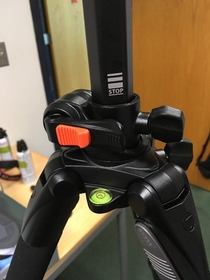
\includegraphics[scale=2]{Lock_1}
\caption{Position the tripod}
\label{Figure 1}
\end{figure}

\begin{figure}[!htp]
\centering
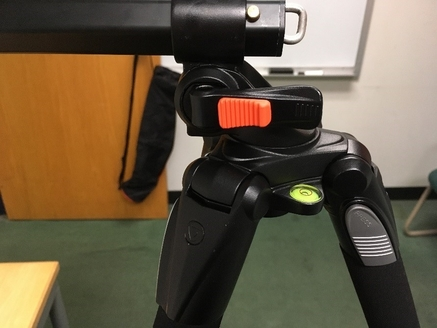
\includegraphics[scale=1.4]{Lock_2}
\caption{Lock the Stand into place}
\label{Figure 2}
\end{figure}

\begin{figure}[!htp]
\centering
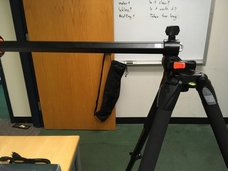
\includegraphics[scale=2.5]{Lock_3}
\caption{Extend the arm over the work area}
\label{Figure 3}
\end{figure}

\newpage

3. Each piece of spike tape will be labeled. Position each item on its corresponding mark. Items with multiple legs will have each leg marked with its location (ie. tripod leg one corresponds to the spike mark labeled "tripod leg 1".) 

4. Plug the shop light and the desk light into the power strip and turn them on. The knight stick and the desk lamp will need to be switched on via their individual on buttons, but the shop light will come on once plugged in. 

5. Before attaching and correctly positioning the camera on the tripod, retrieve the USB cable. The USB cable has plastic piece with screw on one end that attaches to the camera.

6.	Plug in the USB cable to the camera (plug is located on the left side of the camera) and tighten the small screw into the hole found just below the USB plug in. Make sure not to force anything. 

7.	The Camera has an attachment point on its base to screw in a small square piece (Figure 4), the shoe. This will be the attachment point for the tripod. Do not force the screw into the camera!!!

\begin{figure}[!htp]
\centering
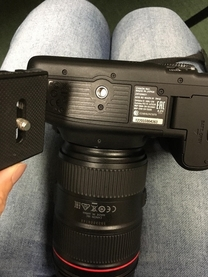
\includegraphics[scale=2]{Camera__2_}
\caption{Camera attachment point}
\label{img:Image 4}
\end{figure}

\newpage

8. Locate the attachment point on the end of the tripod arm. Making sure that the counter weight is present on the backside of the tripod, press the orange button and slide the camera into place. There will be a small click when the camera is in place (Figure 5). 

\begin{figure}[!htp]
\centering
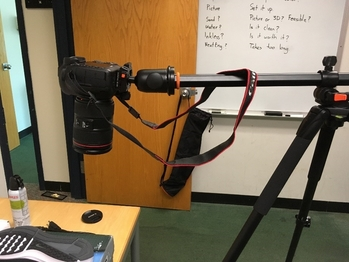
\includegraphics[scale=1.9]{Full_Set_Up}
\caption{Full camera set up}
\label{Image 5}
\end{figure}


9. Making sure that the camera is off, plug the other end of the USB cable into the back of the lap top and remove the lens cap.



\subsection{Camera Cart}

1. Locate the computer cart (Figure 6) that has been designated to be used during shoe impression data collection. With it, locate two ratchet straps, rectangles of cardboard, and a rectangle of foam. 

2. Remove the arm that holds the camera from the tripod. Loosen the screw that keeps the arm in place and slowly pull it out. There will be a small, metal, button that catches before the arm can be completely removed. Push it down and finish removing the arm (Figure 6). 

\begin{figure}[!htp]
\centering
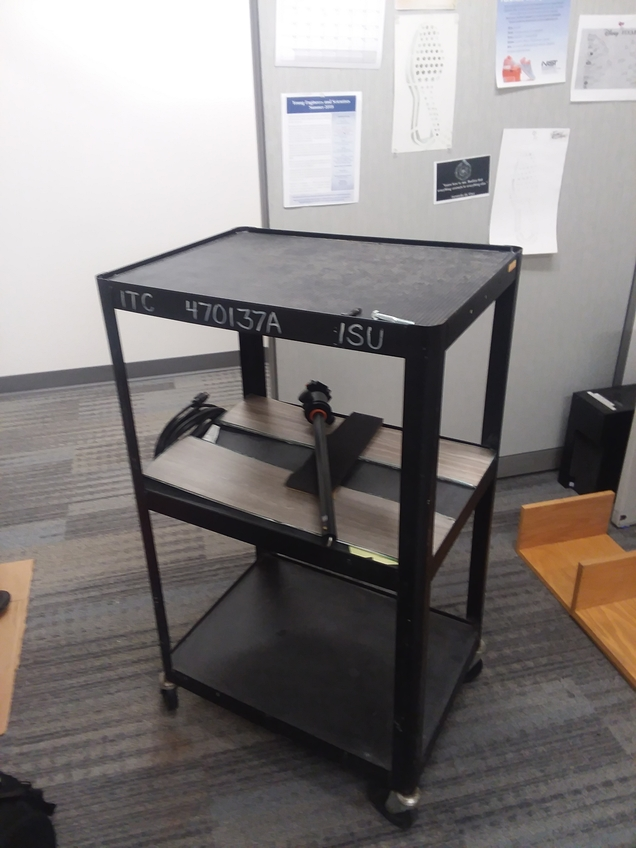
\includegraphics[scale=.2]{CartNew.png}
\caption{An empty computer cart and the arm of the tripod.}
\label{Image 6}
\end{figure}

3. On one of the wide sides of the cart, locate the center of the middle shelf, use the card board to bring the shelf base to just below the lip. Place the foam on top. Once the tripod arm is placed and secured, it should not make contact with the lip of the shelf. 

4. Place the arm on the foam and place small stacks of cardboard length wise just until they get slightly above the base of the arm. This will assist in keeping the arm steady.   

5. At this point, place the ratchet straps around the arm. One will cross the entire shelf near the head of the arm and the other three fourths of the way back on the arm. Secure these straps only until taught (Figure 7). DO NOT OVER TIGHTEN. A third precaution can be taken by tying a chord through the back loop of the arm  and then to the cart itself.  

\begin{figure}[!htp]
\centering
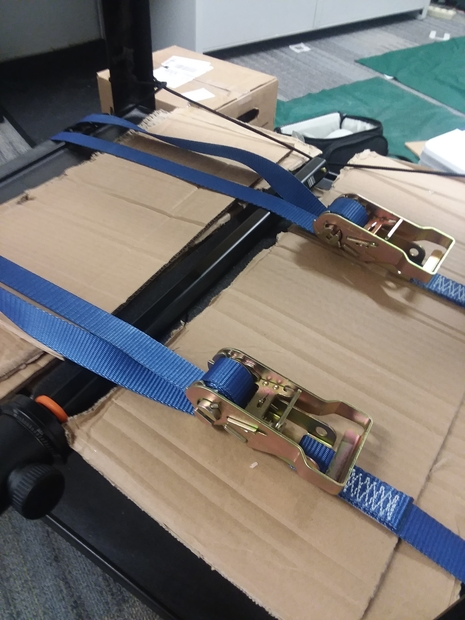
\includegraphics[scale=.28]{Strap.png}
\caption{The tripod arm secured with ratchet straps.}
\label{Image 7}
\end{figure}

\newpage


6. Obtain heavy materials (back-stock dental stone will work) and fill the bottom shelf. This will make sure that the cart does not tip due to the weight of the camera. 

7. Before attaching and correctly positioning the camera on the arm, retrieve the USB cable. The USB cable has a plastic piece with a screw on one end that attaches to the camera.

6.	Plug in the USB cable to the camera (plug is located on the left side of the camera) and tighten the small screw into the hole found just below the USB plug in. Make sure not to force anything. 

7.	The Camera has an attachment point on its base to screw in a small square piece (Figure 8), the shoe. This will be the attachment point for the tripod. Do not force the screw into the camera!!!

\begin{figure}[!htp]
\centering
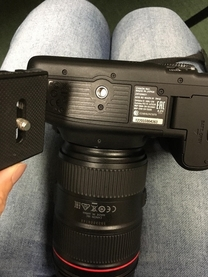
\includegraphics[scale=2]{Camera__2_}
\caption{Camera attachment point}
\label{img:Image 8}
\end{figure}

\newpage

8. Locate the attachment point on the end of the tripod arm.Making sure to support the arm, press the orange button and slide the camera into place. There will be a small click when the camera is in place (Figure 9). Carefully pull your hands away to make sure that the camera is secure. 

\begin{figure}[!htp]
\centering
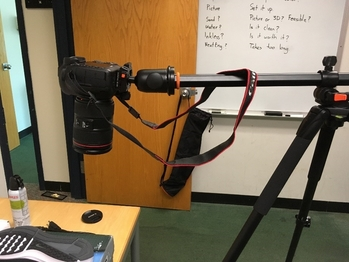
\includegraphics[scale=1.9]{Full_Set_Up}
\caption{Full camera set up}
\label{Image 9}
\end{figure}

9. Place the lap top on the top shelf of the cart and plug the USB end of the camera cord into the back of the laptop (Figure 10-11). 

\begin{figure}[!htp]
\centering
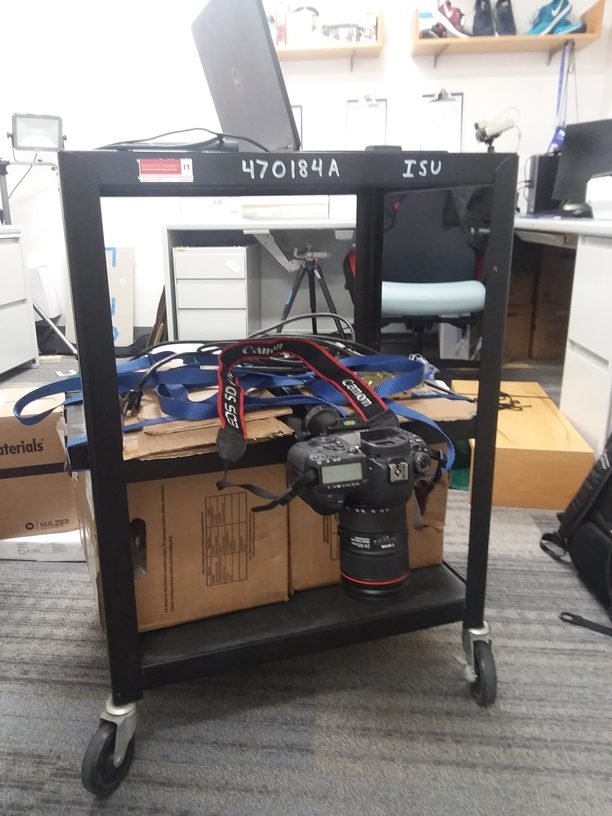
\includegraphics[scale=.2]{Cart1.png}
\caption{Constructed Camera Cart}
\label{Image 10}
\end{figure}

\begin{figure}[!htp]
\centering
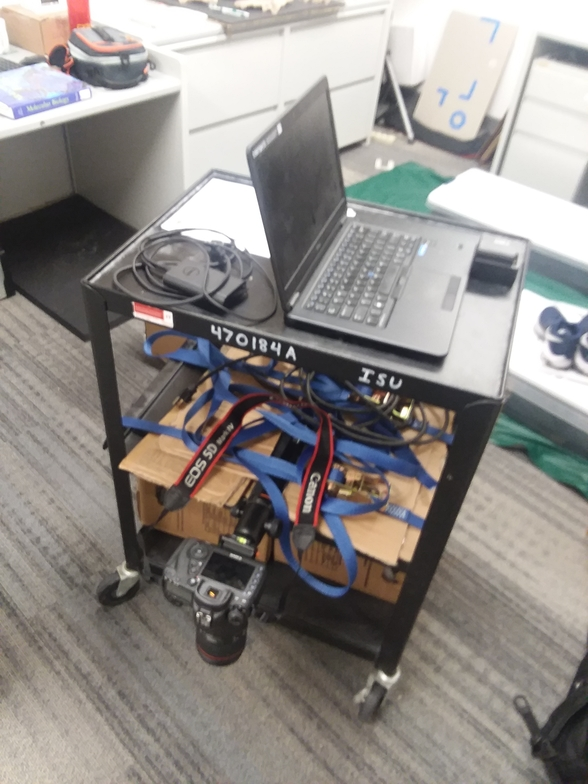
\includegraphics[scale=.2]{Cart2.png}
\caption{Constructed Camera Cart}
\label{Image 11}
\end{figure}

Note: Be careful when using this equipment as you can easily break the camera. 


\subsection{Computer}

1. Turn on the camera by sliding the switch located on the upper left-hand side of the camera from Off to On

2. The computer currently opens the following:
\begin{itemize}
\item Control panel/hardware and sound/devices and printers/canon EOS 5d mark IV
\begin{itemize}
\item this window can be closed
\end{itemize}
\item EOS utility 3
\begin{itemize}
\item if this program does not start you can manually start it
\end{itemize}
\end{itemize}


3. To remotely take pictures, select “remote shooting”
\begin{itemize}
\item This allows for steadier shot when positioned on tripod.
\item To focus, use the mouse to click on the image of the shoe.
\end{itemize}

4. The pop up that comes up is used to control the camera. Select “live view” on this same menu
\begin{itemize}
\item This will bring up live view of the camera in separate pop up from the controls.
\end{itemize}

5. Place the shoe into the box stand with the toe pointing towards the shop light. Place the "L" ruler on the far side of the shoe and bring the stand ruler to the level of the shoe sole. 

6. Place the tag with the correct date and shoe number in the upper left hand corner of the box. Use the bubble level to make sure that the sole of the shoe is completely level.

7. Now, using the live view on the laptop, make sure that the shoe, both scales, and the tag are all visible in the shot.

8. Lastly, before taking the photo. Make sure that all lights are facing the correct direction. The direction of each light is marked with spike tape.
\begin{itemize}
\item The shop light has spike tape on each handle, marking were it should be facing for what image. 
\item For the first image, have the handle marked one directly across from the dot marked one on the tripod (leg 1). Cover the other light with the provided white box. 
\item For the second image, have the handle marked two directly across from the dot marked two on the backboard. 
\end{itemize}

9. Once the photo has been taken, two images will come up for each one image taken. 

\subsection{Saving Photos: Photo Procedure}

1. Select save image and select the non-jpg file. Save this as a Tiff file to the correct location. 

2. Use the naming tool to generate the name for the image file. The Key is on the back of the cover of this manual. Save the completed images (Figure 12-13).

\begin{figure}[!htp]
\centering
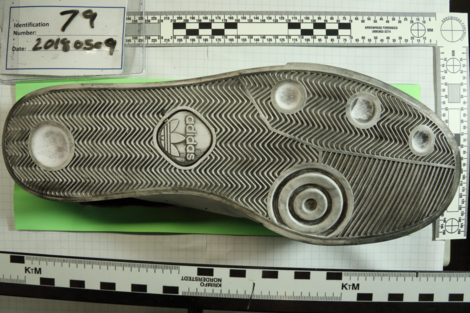
\includegraphics[scale=2.0]{New_photo__2_}
\caption{Example of a good Photo}
\label{Image 12}
\end{figure}

\begin{figure}[!htp]
\centering
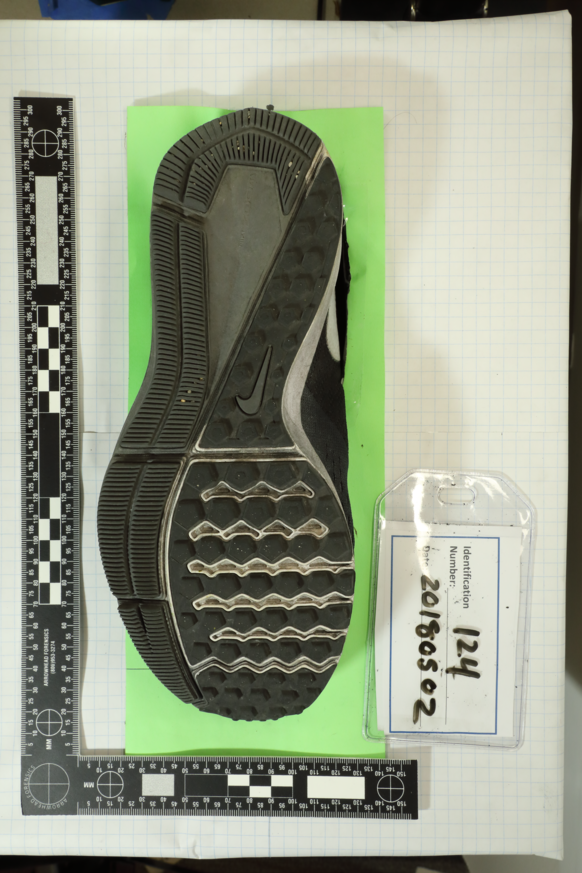
\includegraphics[scale=1.1, angle=90]{New_Photo}
\caption{Example of a good Photo, but it needs the stand scale and the "L" ruler on the other side}
\label{Image 13}
\end{figure}

\newpage


\subsection{Saving Photos: Vinyl Procedure}

1. Remove the SD card from the camera and insert it into the laptop.

2. Transfer all images to the correct folder and notify Guillermo that the files have been uploaded. 

3. Meet with Guillermo about whether the files will be named by hand or with python. 

3. Once all images have been named, transfered, and recorded, please clear the card and re-insert  it into the camera. 


\end{document}